\section{Method}

\begin{figure}[th]
    \vspace{-0.5cm}
    \centering
    % 裁剪图片边缘可能存在的白色区域（根据实际情况调整参数）
        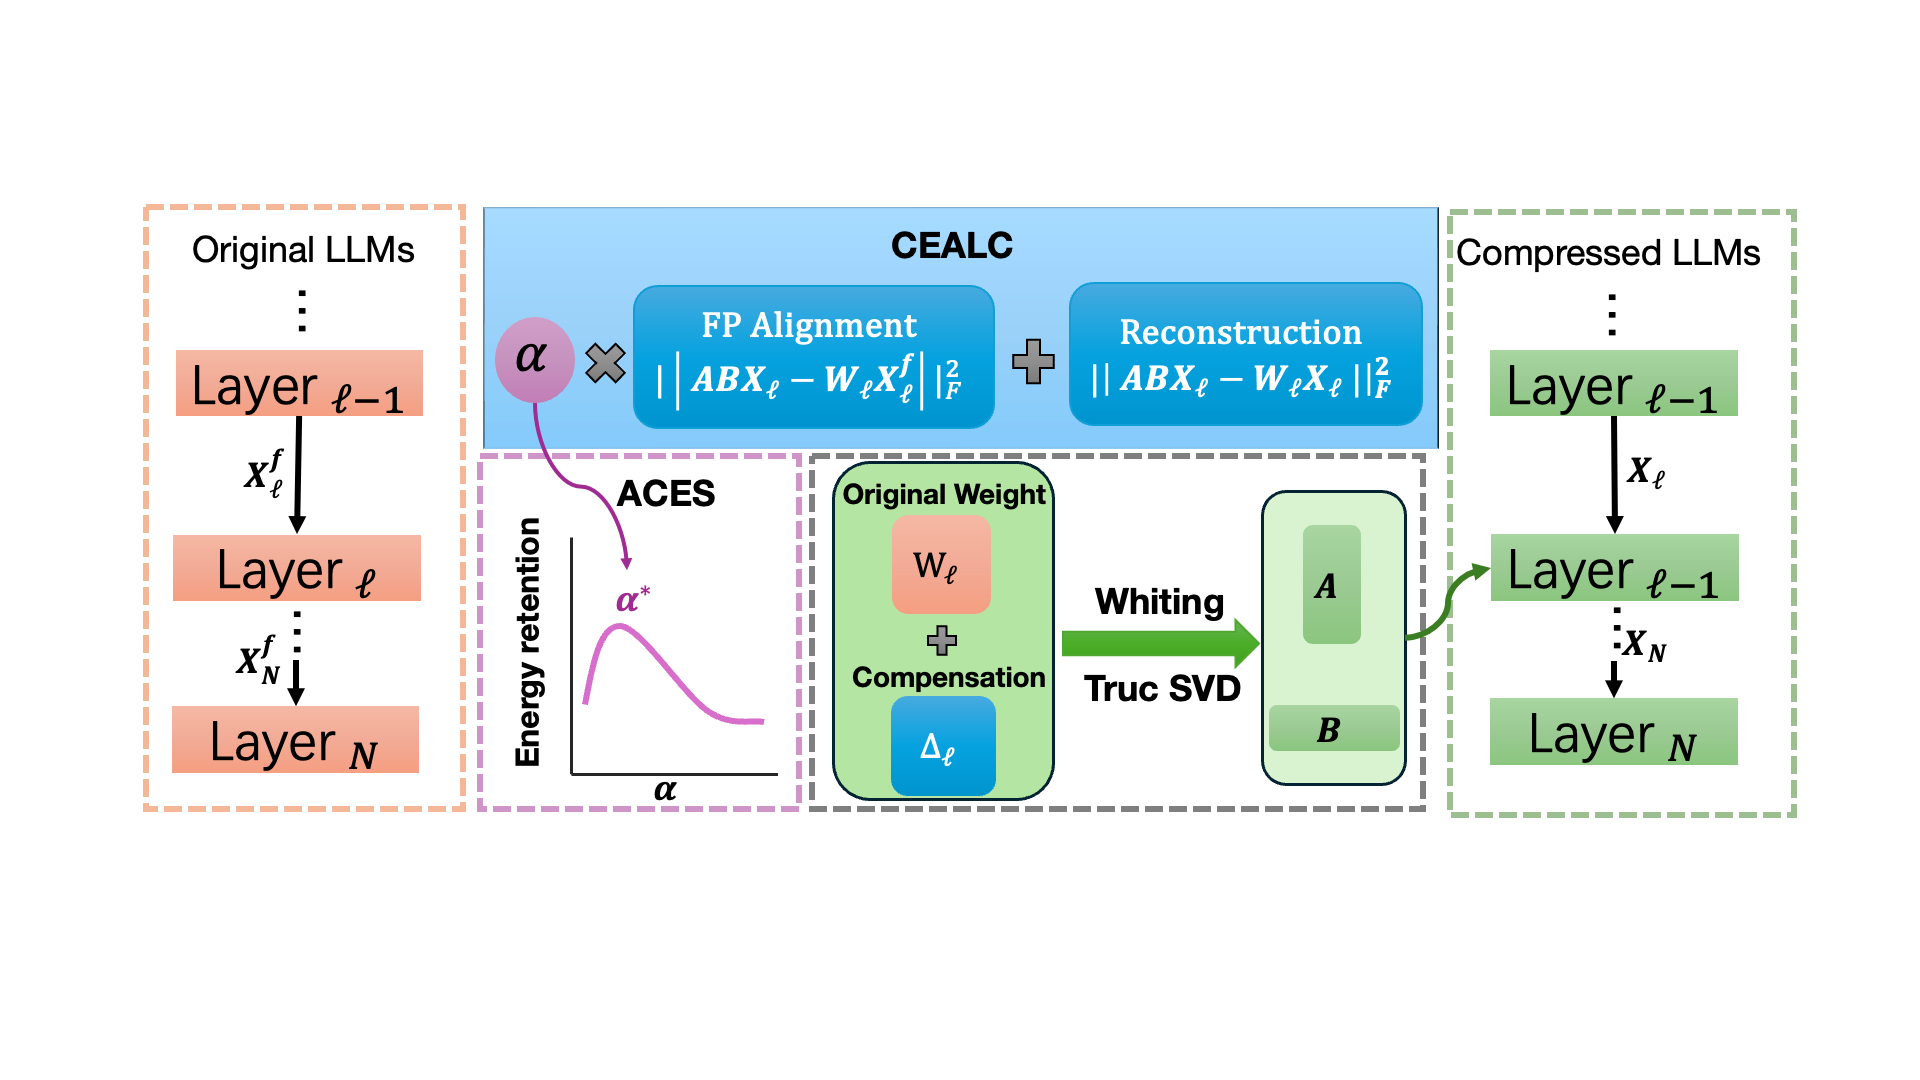
\includegraphics[width=1\linewidth, trim=55 60 55 60, clip]{figs/main.png}
    % 调整标题与图片的距离
    \vspace{-1.5cm}
    \caption{Overview of the proposed SAES-SVD framework.}
    \label{fig:main}  % 标签使用冒号分隔符，符合LaTeX规范
    % 调整图与下文的距离
    \vspace{-0.2cm}
    \end{figure}
We propose SAES-SVD, a unified low-rank compression framework that suppresses both per-layer's reconstruction errors and cumulative deviations accumulated from compressed upstream layers. As illustrated in Figure~\ref{fig:main}, the framework comprises two key components. The first, Cumulative Error-Aware Layer Compression (CEALC), explicitly incorporates cumulative errors compensation into the compression objective, ensuring that each layer aligns closely with its full-precision counterpart. The second, Adaptive Collaborative Error Suppression (ACES), introduces an adaptive coefficient $\alpha$ to balance local reconstruction fidelity with alignment to the full-precision counterpart. The optimal $\alpha$ is chosen to maximize the proportion of retained energy within the truncated subspace.
\subsection{Cumulative Error-
Aware Layer Compression}

\paragraph{Layer compression objective with cumulative error awareness}\label{sec:cealc}
Traditional SVD-based compression methods~\citep{li2025adasvd,Wang2024SVD-LLM} typically approximates the output of the current layer’s weight matrix on its input $X_\ell$ by minimizing Equation~\ref{layerwise svd}. However, this approach neglects cumulative errors propagated from upstream compressed layers, which accumulate with increasing depth and amplify the global deviation from the full-precision (FP) baseline. To address this issue, we introduce an additional alignment term with respect to the FP reference output, leading to the following weighted objective:
\begin{equation}
    \arg\min_{A_\ell,B_\ell}\ \underbrace{\|(A_\ell B_\ell - W_\ell)X_\ell\|_F^2}_{\text{intra-layer
reconstruction
error}} \;+\; \alpha_\ell\,\underbrace{\|A_\ell B_\ell X_\ell - W_\ell X_\ell^f\|_F^2}_{\text{FP reference alignment}}~.
\label{eq:initial}
\end{equation}
Here, $\alpha_\ell \geq 0$ controls the alignment strength. Let $T_\ell = W_\ell X_\ell$ be the original output under current inputs and $R_\ell = W_\ell X_\ell^f$ under FP inputs. Then Equation~\ref{eq:initial} is equivalent to
\begin{equation}
\|(A_\ell B_\ell X_\ell - T_\ell)\|_F^2 + \alpha_\ell \|(A_\ell B_\ell X_\ell - R_\ell)\|_F^2
=(1+\alpha_\ell)\,\|A_\ell B_\ell X_\ell - Z_\ell\|_F^2 + C_\ell,
\label{eq:complete-square}
\end{equation}
where the constant
\(C_\ell := \|T_\ell\|_F^2+\alpha_\ell\|R_\ell\|_F^2-(1+\alpha_\ell)\|Z_\ell\|_F^2\)
is independent of \(A_\ell,B_\ell\), and
\begin{equation}
{
Z_\ell \;=\; \frac{T_\ell+\alpha_\ell R_\ell}{1+\alpha_\ell}
\;=\;
W_\ell\,\frac{X_\ell+\alpha_\ell X_\ell^f}{1+\alpha_\ell}.
}
\label{eq:Z-def}
\end{equation}
Therefore, Equation~\ref{eq:initial} is equivalent to
\begin{equation}
\min_{A_\ell,B_\ell}\ \|A_\ell B_\ell X_\ell - Z_\ell\|_F^2.
\label{eq:reduced-objective}
\end{equation}

% 2.  公式推导
\begin{theorem}\label{theorem 1}
\label{thm:whiten}
As illustrated by the detailed derivation in the Appendix~\ref{theorem1 derivation}, let \(H_{\ell}=X_\ell X_\ell^\top\succ0\) and \(L_\ell=H_{\ell}^{-1/2}\).
Then, for any rank constraint $r_\ell$,
\begin{equation}
\arg\min_{\operatorname{rank}(U_\ell)\le r_\ell}\ \|U_\ell X_\ell - Z_\ell\|_F^2
\;=\;
\arg\min_{\operatorname{rank}(V_\ell)\le r_\ell}\ \big\|V_\ell - M_\ell L_\ell \big\|_F^2,
\quad
\text{with } V_\ell := U_\ell H_{\ell}^{1/2}.
\label{eq:whitened}
\end{equation}
\end{theorem}

Combined with Theorem~\ref{theorem 1}, Equation~\ref{eq:reduced-objective} is equivalent to
\begin{equation}
    \arg\min_{A,B} \Vert ABL^{-1}-ZX^{\top}L\Vert_F^2
\label{eq:l}
\end{equation}
    
\paragraph{Eliminating explicit inputs via second-order statistics.} Storing raw activations $X_\ell$ and their FP counterparts $X_\ell^f$ requires prohibitive memory overhead. For instance, even with a moderate calibration set of 128 samples and sequence length 2048, the activation storage cost exceeds the parameter size by more than two orders of magnitude, making it infeasible for practical large-scale compression. To address this, we reformulate the objective in terms of compact second-order statistics. Specifically, we define the input covariance $H_\ell = X_\ell X_\ell^\top$ and the differential covariance $\Delta_\ell = (X_\ell^f - X_\ell)X_\ell^\top$, which capture the distributional characteristics and upstream-induced shifts. By substituting $X_\ell^f X_\ell^\top = H_\ell + \Delta_\ell$, we obtain
\begin{equation}
Z_\ell X_\ell^\top
=
\frac{W_\ell \big(X_\ell X_\ell^\top + \alpha_\ell X_\ell^f X_\ell^\top\big)}{1+\alpha_\ell}
=
W_\ell\Big(H_\ell + \beta_\ell \Delta_\ell\Big),
\qquad
\beta_\ell := \frac{\alpha_\ell}{1+\alpha_\ell}\in[0,1).
\label{eq:ZXt-stat}
\end{equation}
Substituting Equation~\ref{eq:l} into Equation~\ref{eq:reduced-objective}, then the optimization objective becomes
\begin{equation}
\arg\min_{A_\ell,B_\ell }\|A_\ell B_\ell H_\ell^{1/2}-W_\ell(H_\ell+\beta \Delta_\ell)H_{\ell}^{-1/2}\|_F^2
\label{eq:final}
\end{equation}
Hence, the target in Equation~\ref{eq:reduced-objective} depends only on $H_\ell$ and $\Delta_\ell$, which avoids explicit storage of $X_\ell$ and $X_\ell^f$. In practice, these two second-order statistics are collected in batches and layer by layer, similar to the strategy used in GPTQ, which greatly reduces space complexity.

\paragraph{Closed-form via truncated SVD.} Letting $T_\ell = A_\ell B_\ell H_{\ell}^{1/2}$, and defining the target matrix $G_\ell=W_\ell(H_\ell+\beta \Delta_\ell)H_{\ell}^{-1/2}$, the Eckart–Young–Mirsky~\citep{Eckart1936} theorem guarantees that the best rank-$r$ approximation of $G_\ell$ is obtained by truncated SVD:
\begin{equation}
    T_l^* = [G_\ell]_{r_\ell} = \tilde{U}_{r_\ell}\,\Sigma_{r_\ell}\, \tilde{V}_{r_\ell}^\top,
        \label{eq:final svd}
\end{equation}
where $\Sigma_{r_\ell}$ contains the top-$r_\ell$ singular values, and $\tilde{U}_{r_\ell},\tilde{V}_{r_\ell}$ are the corresponding left and right singular vectors. Consequently, a closed-form solution for $A_\ell$ and $B_\ell$ is given by
\begin{align}
    A_\ell = \tilde{U}_{r_\ell}\,\Sigma_{r_\ell}^{1/2}~, \qquad B_\ell = \Sigma_{r_\ell}^{1/2}\,\tilde{V}_{r_\ell}^\top\,L_\ell
\end{align}
with $L_\ell = H_{\ell}^{-1/2}$ precomputed from input statistics. 
At this point, we complete the derivation of the closed-form solution of CEALC. As shown in Equation~\ref{eq:final}, the approximation target consists of two weighting terms: $W_{\ell}H_{\ell}$ and $\beta \Delta_{\ell}$. The coefficient $\beta$ controls the strength of compensation for upstream cumulative errors when compressing the current layer $\ell$. After applying the whitening matrix $H^{-1/2}$, a truncated SVD yields the optimal theoretical solution.

% Method 2
\subsection{Adaptive Collaborative Error Suppression}\label{sec:adaptive error supression}
\textbf{Motivation.} 
The formulation in Section~\ref{sec:cealc} assumes that the alignment coefficient $\beta_\ell=\frac{\alpha_\ell}{1+\alpha_\ell}$ is fixed in advance. In practice, however, different layers have different sensitivities to accumulated errors from upstream layers. A single alignment strength can disrupt the low-rank structure of the original weights. As shown in Figure~\ref{fig:sub3}, varying $\beta$ alters the low-rank characteristics of the compression objective in Equation~\ref{eq:final}. An inappropriate choice of $\beta_\ell$ scatters spectral energy into non-dominant components, which in turn reduces compression efficiency.
To address this, we reinterpret Equation~\ref{eq:final} as an approximation problem for the original weight matrix $W_\ell$.
The key motivation is to permit moderate weight deviations, but only when such deviations help
% \begin{wrapfigure}{tr}{0.5\textwidth} % r表示右侧，宽度占版心45%
%     \vspace{-0.2cm}
%     \centering
%     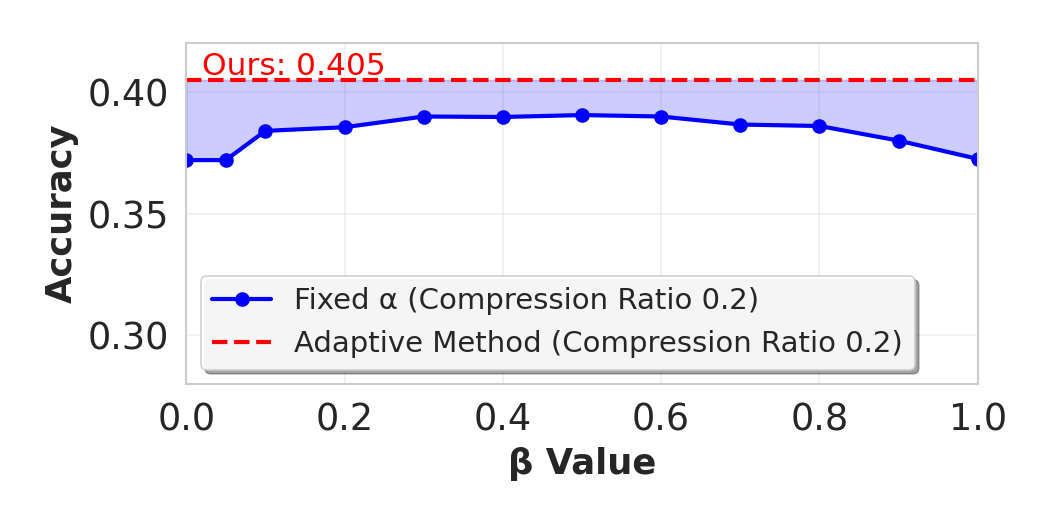
\includegraphics[width=\linewidth, trim=21 21 21 21, clip]{figs/3_plot_different_alpha.png}
%     \vspace{-0.5cm}
%     \caption{Effect of fixed versus adaptive $\beta$ on average accuracy across 7 zero-shot benchmarks. Here, for the sake of convenience, we use the converted $\beta$ as the horizontal axis.}
%     % under different compression ratios.}
%     \vspace{-0.8cm}
%     \label{fig different alpha}
% \end{wrapfigure}

\setlength{\leftmargini}{10pt}
\begin{itemize}
    \item \ding{172} steers the compressed output toward the FP reference, thereby mitigating cumulative error; and 
    \item \ding{173} maximizes the spectral energy preserved in the top-$r_\ell$ singular subspace, avoiding wasteful energy leakage into discarded components.
\end{itemize}
CEALC naturally satisfies condition \ding{172}, where the coefficient $\beta_\ell$ controls the strength of the alignment. Thus, our goal is to determine the optimal $\beta_\ell$ such that, under a rank budget $r_\ell$, the retained subspace preserves as much information as possible. Formally, we define
\begin{equation}
   G_\ell(\beta_\ell) \;=\; S_\ell + \beta_\ell D_\ell,
   \quad 
   \text{with}\;\;
   \begin{cases}
      S_\ell = W_{\ell} H_{\ell} L_{\ell}, \\
      D_\ell = W_{\ell} \Delta_{\ell} L_{\ell}, \\
      \beta_\ell = \dfrac{\alpha_\ell}{1+\alpha_\ell} \in [0,1].
   \end{cases}
\end{equation}
The optimization target can then be expressed as maximizing the proportion of spectral energy captured by the top-$r_\ell$ singular values of $G_\ell(\beta_\ell)$:
\begin{equation}
\label{eq:beta obj}
   \beta_\ell^\star 
   \;=\;
   \arg\max_{\beta_\ell \in [0,1]}
   \frac{ \sum_{i=1}^{r_\ell} \sigma_i^2\!\big(G_\ell(\beta_\ell)\big)}
        { \sum_{i=1}^{\min(m_\ell,n_\ell)} \sigma_i^2\!\big(G_\ell(\beta_\ell)\big)},
\end{equation}
where $\sigma_i(\cdot)$ denotes the $i$-th singular value in decending order after SVD. 
\textbf{However, singular values change with $\beta$, and each trial value would require a new SVD computation, making direct optimization intractable.}
\begin{theorem}[First-Order Approximation of Fixed Subspace(FS-FOA)]
\label{theorem2}
Let $S_\ell \in \mathbb{R}^{m \times n}$ with singular value decomposition
$S_\ell = U_\ell \Sigma_\ell V_\ell^\top$, and let $r_\ell \in \{1,\dots,\min(m,n)-1\}$ be the target rank.  
Denote by $U_{r_\ell} \in \mathbb{R}^{m \times r_\ell}$ and $V_{r_\ell} \in \mathbb{R}^{n \times r_\ell}$ 
the matrices formed by the top-$r_\ell$ left and right singular vectors of $S_\ell$, respectively.  
Define the orthogonal projection matrices
\begin{equation}
P_L^\ell = I - U_{r_\ell} U_{r_\ell}^\top, 
\qquad 
P_R^\ell = I - V_{r_\ell} V_{r_\ell}^\top.
\end{equation}

For $G_\ell(\beta) = S_\ell + \beta D_\ell$,
the relative error ratio can be approximated by
\begin{equation}
   \widetilde\rho_\ell(\beta) \;=\; 
   \frac{\|P_L^\ell\,G_\ell(\beta)\,P_R^\ell\|_F}{\|G_\ell(\beta)\|_F}
   \;=\; 
   \frac{\|S_\ell^\perp + \beta D_\ell^\perp\|_F}{\|S_\ell + \beta D_\ell\|_F},
\end{equation}
    where $S_\ell^\perp = P_L^\ell S_\ell P_R^\ell$ and $D_\ell^\perp = P_L^\ell D_\ell P_R^\ell$ are the projections of $S_\ell$ and $D_\ell$ onto the orthogonal complements of the top-$r_\ell$ singular subspaces of $S_\ell$. Detailed proof can be referred to Appendix \ref{theorem2 derivation}.
\end{theorem}

For computational tractability, we freeze the principal subspace at $\beta=0$, leveraging Theorem\ref{theorem2}. The resulting approximation ratio can be written as
\begin{equation}
    \widetilde\rho(\beta) = \frac{\|S_\ell^\perp + \beta D_\ell^\perp\|_F^2}{\|S_\ell + \beta D_\ell\|_F^2} = \frac{a + 2b\,\beta + c\,\beta^2}{A + 2B\,\beta + C\,\beta^2}~,
\end{equation}
where
\begin{equation}
a=\left\|{S_\ell}_{\perp}\right\|_F^2, \quad b=\left\langle {S_\ell}_{\perp}, {D_\ell}_{\perp}\right\rangle, \quad c=\left\|{D_\ell}_{\perp}\right\|_F^2, \quad A=\|{S_\ell}|_F^2, \quad B=\langle {S_\ell}, {D_\ell}\rangle, \quad C=\|{D_\ell}\|_F^2
\end{equation}
Setting the derivative of $\widetilde\rho(\beta)$ to zero yields a quadratic equation
\begin{equation}
    \widetilde{p}(\beta) = (cB - bC)\,\beta^2 + (cA - aC)\,\beta + (bA - aB) = 0\,.
    \label{eq: beta compute}
\end{equation}
We evaluate all real roots within a feasible interval $[\beta{\min},\beta_{\max}]$ (e.g., $[0,1]$), along with the endpoints and the minimizer $\beta^\star$ of $\widetilde\rho(\beta)$ is then selected. This adaptive selection minimizes the fraction of truncated energy, ensuring that the retained singular spectrum captures the maximum proportion of information. 
As illustrated in Figure~\ref{fig different alpha}, the adaptive strategy consistently outperforms fixed-$\alpha$ settings across different compression ratios, highlighting both its robustness and effectiveness. 

Through CEALC and ACES, we establish a closed-loop compression mechanism: each layer adaptively selects $\alpha_\ell$ to suppress newly introduced truncation error, while residual error is accumulated into second-order statistics and propagated forward. This allows subsequent layers to anticipate and compensate for upstream cumulative errors. Consequently, the model achieves output fidelity close to the baseline using only a single SVD approximation per layer. The detailed implementation can be found in Appendix \ref{appendix:algorithm}.